\chapter{Numbers 18}

\begin{figure}
  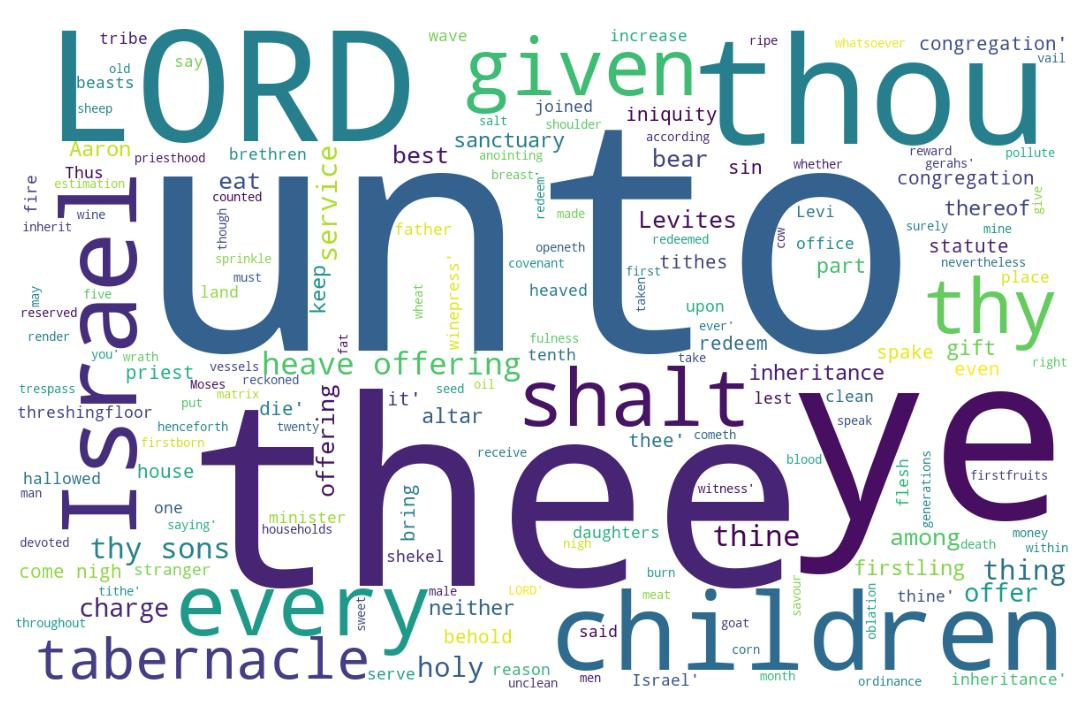
\includegraphics[width=\linewidth]{04OT-Numbers/Numbers18-WordCloud.jpg}
  \caption{Numbers 18 Word Cloud}
  \label{fig:Numbers 18 word Cloud}
\end{figure}


\marginpar{\scriptsize \centering \fcolorbox{bone}{lime}{\textbf{THE AARONIC PRIESTHOOD}}\\ (Numbers 18:1-32) \begin{compactenum}[I.][8]
    \item  \textbf{Sanctuary} \index[scripture]{Numbers!Num 18:01} \index[scripture]{Numbers!Num 18:03}\index[scripture]{Numbers!Num 18:05}\index[scripture]{Numbers!Num 18:16}(Numbers 18:1, 3, 5, 16) -- access to the sanctuary
    \item  \textbf{Sons} \index[scripture]{Numbers!Num 18:01} \index[scripture]{Numbers!Num 18:02}\index[scripture]{Numbers!Num 18:07}\index[scripture]{Numbers!Num 18:08}\index[scripture]{Numbers!Num 18:09}\index[scripture]{Numbers!Num 18:11}\index[scripture]{Numbers!Num 18:19} (Numbers 18:1, 2, 7, 8, 9, 11, 19) -- there is a family relationship between the priests. Here is the Aaronic priesthood. Elsewhere, see the priesthood of Melchisedek!
    \item  \textbf{Service} \index[scripture]{Numbers!Num 18:04} \index[scripture]{Numbers!Num 18:06}\index[scripture]{Numbers!Num 18:07}\index[scripture]{Numbers!Num 18:21}\index[scripture]{Numbers!Num 18:31}(Numbers 18:4, 6, 7, 21, 23, 31) -- the priests had duties of service
    \item  \textbf{Strangers} \index[scripture]{Numbers!Num 18:04} \index[scripture]{Numbers!Num 18:07}  (Numbers 18:4, 7) -- The strangers, people not part of God's fold, have no business with the priesthood
    \item  \textbf{Statutes} \index[scripture]{Numbers!Num 18:11} \index[scripture]{Numbers!Num 18:19}\index[scripture]{Numbers!Num 18:23} (Numbers 18:11, 19, 23) -- There are rules, God-given rules, for accessing and serving God
    \item  \textbf{Sin \& Sinners} \index[scripture]{Numbers!Num 18:09} \index[scripture]{Numbers!Num 18:22}\index[scripture]{Numbers!Num 18:26} \index[scripture]{Numbers!Num 18:32}(Numbers 18:9, 22, 26, 32) -- That sin problem -- always there to be dealt with
\end{compactenum}}
    




\footnote{\textcolor[cmyk]{0.99998,1,0,0}{\hyperlink{TOC}{Return to end of Table of Contents.}}}\footnote{\href{https://audiobible.com/bible/numbers_18.html}{\textcolor[cmyk]{0.99998,1,0,0}{Numbers 18 Audio}}}\textcolor[cmyk]{0.99998,1,0,0}{And the LORD said unto Aaron, Thou and thy \fcolorbox{bone}{lime}{sons} and thy father's house with thee shall bear the iniquity of the \fcolorbox{bone}{lime}{sanctuary}: and thou and thy sons with thee shall bear the iniquity of your priesthood.}
[2] \textcolor[cmyk]{0.99998,1,0,0}{And thy brethren also of the tribe of Levi, the tribe of thy father, bring thou with thee, that they may \fcolorbox{bone}{bone}{be} joined unto thee, and minister unto thee: but thou and thy \fcolorbox{bone}{lime}{sons} with thee \emph{shall} \emph{minister} before the tabernacle of witness.}
[3] \textcolor[cmyk]{0.99998,1,0,0}{And they shall keep thy charge, and the charge of all the tabernacle: only they shall not come nigh the vessels of the \fcolorbox{bone}{lime}{sanctuary} and the altar, that neither they, nor ye also, die.}
[4] \textcolor[cmyk]{0.99998,1,0,0}{And they shall \fcolorbox{bone}{bone}{be} joined unto thee, and keep the charge of the tabernacle of the congregation, for all the \fcolorbox{bone}{lime}{service} of the tabernacle: and \fcolorbox{bone}{bone}{a} \fcolorbox{bone}{lime}{stranger} shall not come nigh unto you.}
[5] \textcolor[cmyk]{0.99998,1,0,0}{And ye shall keep the charge of the \fcolorbox{bone}{lime}{sanctuary}, and the charge of the altar: that there \fcolorbox{bone}{bone}{be} no wrath any more upon \fcolorbox{bone}{bone}{the children of Israel}.}
[6] \textcolor[cmyk]{0.99998,1,0,0}{And \fcolorbox{bone}{bone}{I}, behold, \fcolorbox{bone}{bone}{I} have taken your brethren the Levites from among \fcolorbox{bone}{bone}{the children of Israel}: to you \emph{they} \emph{are} given \emph{as} \fcolorbox{bone}{bone}{a} gift for the LORD, to do the \fcolorbox{bone}{lime}{service} of the tabernacle of the congregation.}
[7] \textcolor[cmyk]{0.99998,1,0,0}{Therefore thou and thy \fcolorbox{bone}{lime}{sons} with thee shall keep your priest's office for every thing of the altar, and within the vail; and ye shall serve: \fcolorbox{bone}{bone}{I} have given your priest's office \emph{unto} \emph{you} as \fcolorbox{bone}{bone}{a} \fcolorbox{bone}{lime}{service} of gift: and the \fcolorbox{bone}{lime}{stranger} that cometh nigh shall \fcolorbox{bone}{bone}{be} put to death.}\\
\\
\P \textcolor[cmyk]{0.99998,1,0,0}{And the LORD spake unto Aaron, Behold, \fcolorbox{bone}{bone}{I} also have given thee the charge of mine heave offerings of all the hallowed things of \fcolorbox{bone}{bone}{the children of Israel}; unto thee have \fcolorbox{bone}{bone}{I} given them by reason of the anointing, and to thy \fcolorbox{bone}{lime}{sons}, by an ordinance for ever.}
[9] \textcolor[cmyk]{0.99998,1,0,0}{This shall \fcolorbox{bone}{bone}{be} thine of the most holy things, \emph{reserved} from the fire: every oblation of their's, every meat offering of their's, and every \fcolorbox{bone}{lime}{sin} offering of their's, and every trespass offering of their's, which they shall render unto me, \emph{shall} \emph{be} most holy for thee and for thy \fcolorbox{bone}{lime}{sons}.}
[10] \textcolor[cmyk]{0.99998,1,0,0}{In the most holy \emph{place} shalt thou eat it; every male shall eat it: it shall \fcolorbox{bone}{bone}{be} holy unto thee.}
[11] \textcolor[cmyk]{0.99998,1,0,0}{And this \emph{is} thine; the heave offering of their gift, with all the wave offerings of \fcolorbox{bone}{bone}{the children of Israel}: \fcolorbox{bone}{bone}{I} have given them unto thee, and to thy \fcolorbox{bone}{lime}{sons} and to thy daughters with thee, by \fcolorbox{bone}{bone}{a} \fcolorbox{bone}{lime}{statute} for ever: every one that is clean in thy house shall eat of it.}
[12] \textcolor[cmyk]{0.99998,1,0,0}{All the best of the oil, and all the best of the wine, and of the wheat, the firstfruits of them which they shall offer unto the LORD, them have \fcolorbox{bone}{bone}{I} given thee.}
[13] \textcolor[cmyk]{0.99998,1,0,0}{\emph{And} whatsoever is first ripe in the land, which they shall bring unto the LORD, shall \fcolorbox{bone}{bone}{be} thine; every one that is clean in thine house shall eat \emph{of} it.}
[14] \textcolor[cmyk]{0.99998,1,0,0}{Every thing devoted in Israel shall \fcolorbox{bone}{bone}{be} thine.}
[15] \textcolor[cmyk]{0.99998,1,0,0}{Every thing that openeth the matrix in all flesh, which they bring unto the LORD, \emph{whether} \emph{it} \emph{be} of men or beasts, shall \fcolorbox{bone}{bone}{be} thine: nevertheless the firstborn of man shalt thou surely redeem, and the firstling of unclean beasts shalt thou redeem.}
[16] \textcolor[cmyk]{0.99998,1,0,0}{And those that are to \fcolorbox{bone}{bone}{be} redeemed from \fcolorbox{bone}{bone}{a} month old shalt thou redeem, according to thine estimation, for the money of five shekels, after the shekel of the \fcolorbox{bone}{lime}{sanctuary}, which \emph{is} twenty gerahs.}
[17] \textcolor[cmyk]{0.99998,1,0,0}{But the firstling of \fcolorbox{bone}{bone}{a} cow, or the firstling of \fcolorbox{bone}{bone}{a} sheep, or the firstling of \fcolorbox{bone}{bone}{a} goat, thou shalt not redeem; they \emph{are} holy: thou shalt sprinkle their blood upon the altar, and shalt burn their fat \emph{for} an offering made by fire, for \fcolorbox{bone}{bone}{a} sweet savour unto the LORD.}
[18] \textcolor[cmyk]{0.99998,1,0,0}{And the flesh of them shall \fcolorbox{bone}{bone}{be} thine, as the wave breast and as the right shoulder are thine.}
[19] \textcolor[cmyk]{0.99998,1,0,0}{All the heave offerings of the holy things, which \fcolorbox{bone}{bone}{the children of Israel} offer unto the LORD, have \fcolorbox{bone}{bone}{I} given thee, and thy \fcolorbox{bone}{lime}{sons} and thy daughters with thee, by \fcolorbox{bone}{bone}{a} \fcolorbox{bone}{lime}{statute} for ever: it \emph{is} \fcolorbox{bone}{bone}{a} covenant of salt for ever before the LORD unto thee and to thy seed with thee.}\\
\\
\P \textcolor[cmyk]{0.99998,1,0,0}{And the LORD spake unto Aaron, Thou shalt have no inheritance in their land, neither shalt thou have any part among them: \fcolorbox{bone}{bone}{I} \emph{am} thy part and thine inheritance among \fcolorbox{bone}{bone}{the children of Israel}.}
[21] \textcolor[cmyk]{0.99998,1,0,0}{And, behold, \fcolorbox{bone}{bone}{I} have given the children of Levi all the tenth in Israel for an inheritance, for their service which they serve, \emph{even} the \fcolorbox{bone}{lime}{service} of the tabernacle of the congregation.}
[22] \textcolor[cmyk]{0.99998,1,0,0}{Neither must \fcolorbox{bone}{bone}{the children of Israel} henceforth come nigh the tabernacle of the congregation, lest they bear \fcolorbox{bone}{lime}{sin}, and die.}
[23] \textcolor[cmyk]{0.99998,1,0,0}{But the Levites shall do the \fcolorbox{bone}{lime}{service} of the tabernacle of the congregation, and they shall bear their iniquity: \emph{it} \emph{shall} \emph{be} \fcolorbox{bone}{bone}{a} \fcolorbox{bone}{lime}{statute} for ever throughout your generations, that among \fcolorbox{bone}{bone}{the children of Israel} they have no inheritance.}
[24] \textcolor[cmyk]{0.99998,1,0,0}{But the tithes of \fcolorbox{bone}{bone}{the children of Israel}, which they offer \emph{as} an heave offering unto the LORD, \fcolorbox{bone}{bone}{I} have given to the Levites to inherit: therefore \fcolorbox{bone}{bone}{I} have said unto them, Among \fcolorbox{bone}{bone}{the children of Israel} they shall have no inheritance.}\\
\\
\P \textcolor[cmyk]{0.99998,1,0,0}{And the LORD spake unto Moses, saying,}
[26] \textcolor[cmyk]{0.99998,1,0,0}{Thus speak unto the Levites, and say unto them, When ye take of \fcolorbox{bone}{bone}{the children of Israel} the tithes which \fcolorbox{bone}{bone}{I} have given you from them for your inheritance, then ye shall offer up an heave offering of it for the LORD, \emph{even} \fcolorbox{bone}{bone}{a} tenth \emph{part} of the tithe.}
[27] \textcolor[cmyk]{0.99998,1,0,0}{And \emph{this} your heave offering shall \fcolorbox{bone}{bone}{be} reckoned unto you, as though \emph{it} \emph{were} the corn of the threshingfloor, and as the fulness of the winepress.}
[28] \textcolor[cmyk]{0.99998,1,0,0}{Thus ye also shall offer an heave offering unto the LORD of all your tithes, which ye receive of \fcolorbox{bone}{bone}{the children of Israel}; and ye shall give thereof the LORD'S heave offering to Aaron the priest.}
[29] \textcolor[cmyk]{0.99998,1,0,0}{Out of all your gifts ye shall offer every heave offering of the LORD, of all the best thereof, \emph{even} the hallowed part thereof out of it.}
[30] \textcolor[cmyk]{0.99998,1,0,0}{Therefore thou shalt say unto them, When ye have heaved the best thereof from it, then it shall \fcolorbox{bone}{bone}{be} counted unto the Levites as the increase of the threshingfloor, and as the increase of the winepress.}
[31] \textcolor[cmyk]{0.99998,1,0,0}{And ye shall eat it in every place, ye and your households: for it \emph{is} your reward for your \fcolorbox{bone}{lime}{service} in the tabernacle of the congregation.}
[32] \textcolor[cmyk]{0.99998,1,0,0}{And ye shall bear no \fcolorbox{bone}{lime}{sin} by reason of it, when ye have heaved from it the best of it: neither shall ye pollute the holy things of \fcolorbox{bone}{bone}{the children of Israel}, lest ye die.}